\chapter{并发控制}

\begin{introduction}[期末考试提纲]
  \item X锁、S锁、U锁、IS锁、IX锁、SIX锁
  \item 两段锁协议内容及其作用
  \item 死锁及其解决措施
  \item 基于时间戳的并发控制协议
  \item 基于有效性检查的并发控制协议
  \item MySQL MVCC中的读视图和可见性算法
\end{introduction}

\section{基于锁的协议}

\begin{definition}[封锁]
  \textcolor{red}{封锁}就是一个事务对某个数据对象加锁, 取得对它一定的控制, 限制其它事务对该数据对象使用.
  
  要访问数据项$R$, 事务$T_i$必须先申请对$R$的封锁, 如果$R$已经被事务$T_j$加了不相容的锁, 则$T_i$需要等待, 直至$T_j$释放它的封锁.
\end{definition}

\textcolor{red}{封锁性能}: 事务吞吐量, TPC-C.

\subsection{封锁类型}

\begin{itemize}
  \item 基本锁类型: X锁、S锁、U锁
  \item 意向锁: IS、IX、IU、SIX
  \item 码范围锁: RangeS\_S、RangeI\_N
  \item 其他锁: 模式锁、闩锁、BU锁
\end{itemize}

\begin{definition}[排它锁(X锁, eXclusive lock)]
  lock-X($R$): 又称写锁, 持有X锁可以读写数据项.

  事务$T$对数据对象$R$加上X锁, 则其它事务对$R$的任何封锁请求都
不能成功, 直至$T$释放$R$上的X锁.
\end{definition}

\begin{definition}[共享锁(S锁, Share lock)]
  lock-S($R$): 又称读锁, 持有S
锁只能读取数据项.

事务$T$对数据对象$R$加上X锁, 则其它事务对$R$的任何\textcolor{red}{$X$锁请求}都
不能成功, 而对$R$的S锁请求可以成功.
\end{definition}

封锁的相容矩阵comp(A,B):
\begin{table}[H]
    \centering
    \begin{tabular}{|c|c|c|}
        \hline
        \multirow{2}{*}{\textbf{请求锁模式A}} & \multicolumn{2}{c|}{\textbf{现有锁模式B}} \\ \cline{2-3}
         & \textbf{S} & \textbf{X} \\ \hline
        \textbf{S} & \cellcolor{red!10}\textcolor{blue}{是} & \textcolor{blue}{否} \\ \hline
        \textbf{X} & \textcolor{blue}{否} & \textcolor{blue}{否} \\ \hline
    \end{tabular}
    \caption{封锁的相容矩阵}
    \label{tab:lock_compatibility}
\end{table}

长锁: 保持到事务结束时才释放的锁

短锁: 在事务中途就可以释放的锁

\begin{itemize}
  \item read uncommitted: 不申请锁.
  \item read committed: 短S锁.
  \item repeatable read: 长S锁.
\end{itemize}

\subsection{两阶段封锁协议}

保证可串行化的一种协议是两阶段封锁协议(two-phase Locking protocol). 该协议要求\textbf{每个事务}分两个阶段提出加锁和解锁申请.
\begin{enumerate}
    \item 增长阶段(growing phase): 一个事务可以获得锁, 但不能释放任何锁.
    \item 缩减阶段(shrinking phase): 一个事务可以释放锁, 但不能获得任何新锁.
\end{enumerate}
起初, 一个事务处于增长阶段. 事务根据需要获得锁. 一旦该事务释放了一个锁, 它就进入了缩减阶段, 并且它不能再发出加锁请求.

\begin{definition}[封锁点]
  封锁点: 事务获得其最后封锁的时间.
\end{definition}

\begin{theorem}
  若一组事务均服从两阶段封锁协议, 则它们的调度一定是可串行化的.

  事务调度等价于和其封锁点顺序一致的串行调度.
\end{theorem}

\begin{proof}
  令$\{T_0,T_1,...,T_n\}$是参与调度$S$的事务集. 如果$T_i$对数据项$R$加$A$型锁, $T_j$对数据项$R$加$B$型锁, 且$comp(A,B)=false$. 若$T_i$先于$T_j$, 记作$T_i\to T_j$, 得到一个优先图.

  设$t_i$是$T_i$的封锁点, \textcolor{red}{若$T_i\to T_j$, 则$t_i\to t_j$.}

  若$\{T_0,T_1,...,T_n\}$不可串行化, 则在优先图中存在环, 不妨设为$T_0\to T_1\to \cdots \to T_n \to t_0$, 则$t_0<t_1<\cdots<t_n<t_0$, 矛盾!
\end{proof}

2PL 可以保证调度是可串行化的吗? 可以. 如上.

2PL 可以保证调度是无级联的吗? 不能保证. 在标准的 基本 2PL 中, 一个事务可能读取到另一个尚未提交事务写入的数据(即“脏读”).

\begin{figure}[H]
    \centering
    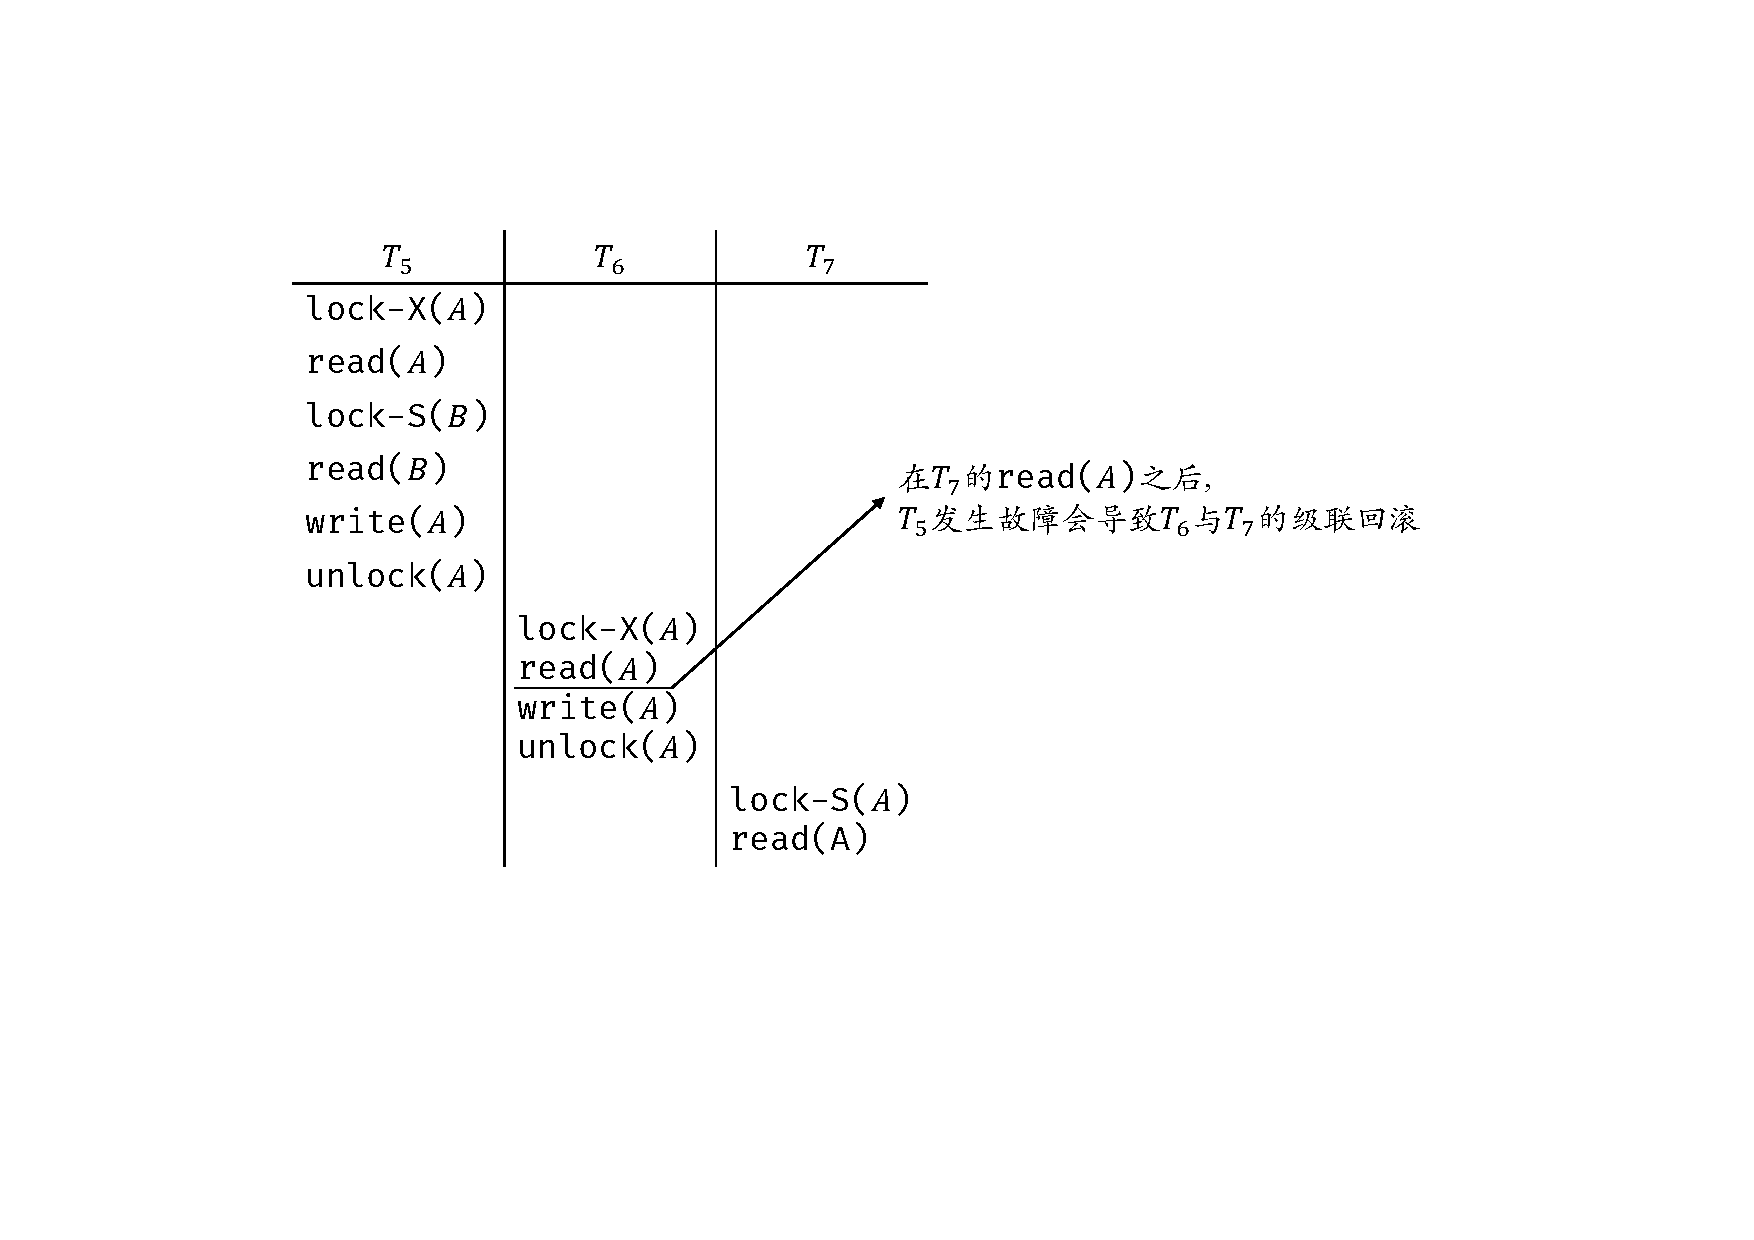
\includegraphics[width=.7\textwidth]{figure/级联.pdf}
    \caption{2PL的级联回滚}
\end{figure}

2PL 可以保证调度避免不可重复读吗? 不一定. 

严格2PL(strict two-phrase locking protocol): 要求X锁是长锁.

严厉2PL(rigorous two-phrase locking protocol): 要求S锁和X锁均是长锁.




